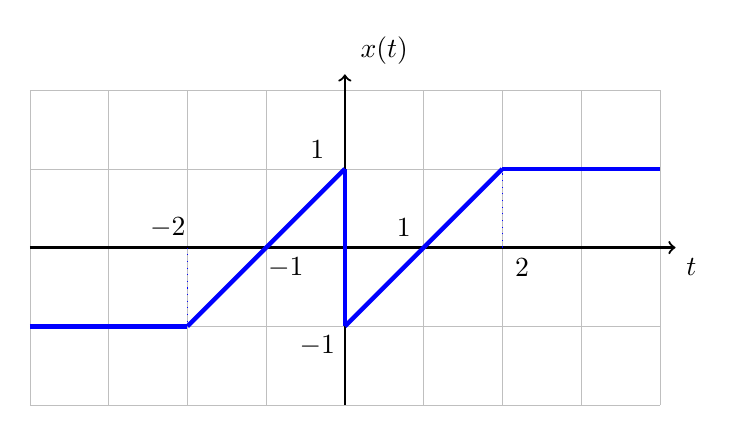
\begin{tikzpicture}

  % -- Dibujamos la cuadrícula
  \draw [lightgray, ultra thin] (-4,-2) grid (4,2);

  % -- Dibujamos los ejes
  \draw [thick][->] (-4,0) -- (4.2,0);
  \draw [thick][->] (0,-2) -- (0,2.2);

  % -- Dibujamos la trayectoria
  \draw [ultra thick, blue] (-4,-1) -- (-2,-1);
  \draw [ultra thick, blue] (-2,-1) -- (0,1);
  \draw [ultra thick, blue] (0,1) -- (0,-1);
  \draw [ultra thick, blue] (0,-1) -- (2,1);
  \draw [ultra thick, blue] (2,1) -- (4,1);
  \draw [dotted, thin, blue] (-2,0) -- (-2,-1);
  \draw [dotted, thin, blue] (2,0) -- (2,1);

  % -- Etiquetamos los ejes y colocamos anotaciones
  \node at (0.5,2.5) {$x(t)$};
  \node at (4.4,-0.25) {$t$};
  \node at (-2.25,0.25) {$-2$};
  \node at (-0.75,-0.25) {$-1$};
  \node at (0.75,0.25) {$1$};
  \node at (2.25,-0.25) {$2$};
  \node at (-0.35,1.25) {$1$};
  \node at (-0.35,-1.25) {$-1$};

\end{tikzpicture}
